\def\chapdir{./Chapter04}

\chapter{System Architecture} \label{ch:system-architecture}

\section{Overall Architecture}

\subsection{High-level System Architecture Overview}

The OllamaNet platform is built on a modern microservices architecture that separates concerns into distinct, independently deployable services. Each service focuses on a specific domain within the system, communicating through well-defined APIs and messaging patterns.

\begin{figure}[p]
    \centering
    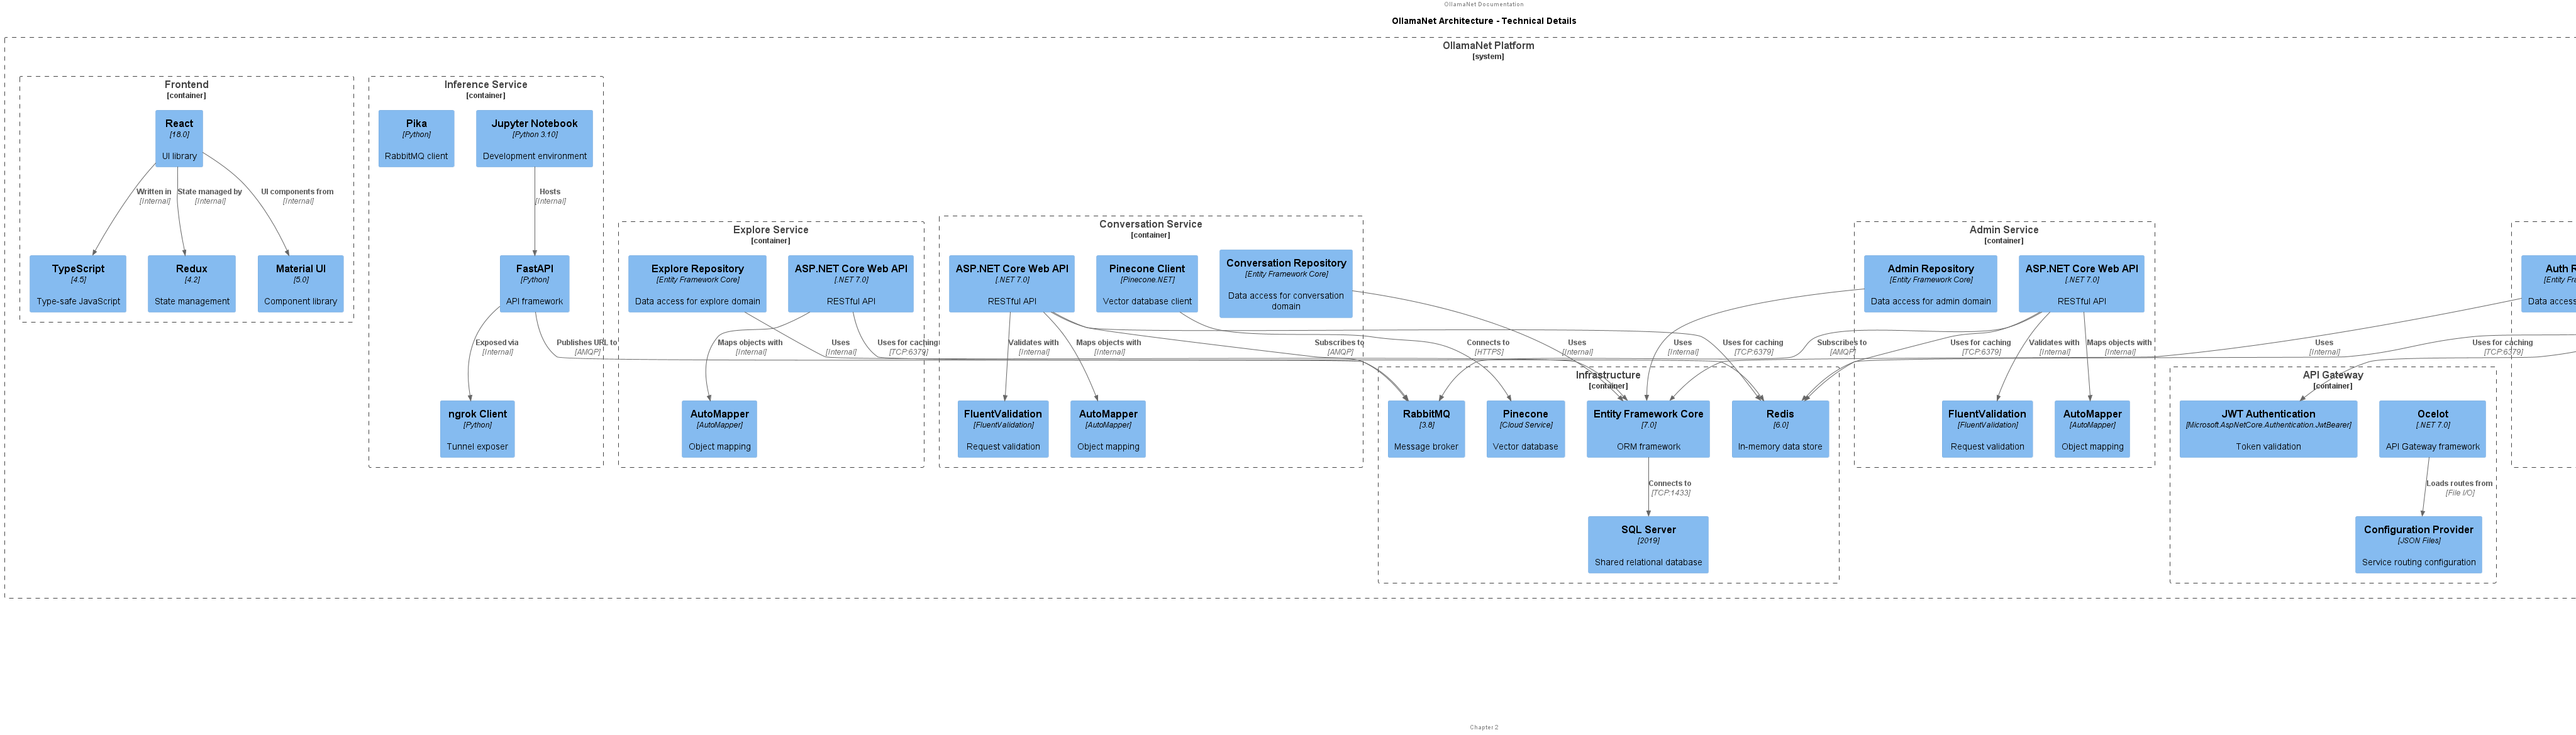
\includegraphics[width=\textwidth]{./Chapter04/figures/OllamaNet_Architecture.png}
    \caption{OllamaNet High-level System Architecture}
    \label{fig:system-architecture}
\end{figure}
\clearpage

The architecture consists of the following key components:

\begin{enumerate}
   \item \textbf{API Gateway}: Serves as the entry point for all client requests, handling routing, authentication, and cross-cutting concerns.
   \item \textbf{Auth Service}: Manages user authentication, authorization, and account management.
   \item \textbf{Admin Service}: Provides administrative capabilities for user and model management.
   \item \textbf{Explore Service}: Enables discovery and browsing of available AI models.
   \item \textbf{Conversation Service}: Handles conversation management and interaction with AI models.
   \item \textbf{Inference Service}: Connects to the Ollama engine for AI model inference.
   \item \textbf{Database Layer}: Provides data persistence across services.
   \item \textbf{RabbitMQ}: Facilitates asynchronous communication and service discovery.
\end{enumerate}

\subsection{Architectural Principles and Goals}

The OllamaNet architecture adheres to the following principles:

\begin{enumerate}
   \item \textbf{Service Independence}: Each service can be developed, deployed, and scaled independently.
   \item \textbf{Domain-Driven Design}: Services are organized around business domains rather than technical functions.
   \item \textbf{API-First Design}: All services expose well-defined APIs with consistent patterns.
   \item \textbf{Resilience by Design}: The system is designed to handle failures gracefully.
   \item \textbf{Security at Every Layer}: Authentication and authorization are enforced consistently.
   \item \textbf{Scalability}: Services can be scaled independently based on demand.
   \item \textbf{Observability}: The system provides monitoring, logging, and diagnostics capabilities.
\end{enumerate}

The architectural goals include:

\begin{enumerate}
   \item \textbf{Maintainability}: Clear separation of concerns makes the system easier to maintain.
   \item \textbf{Extensibility}: New features can be added with minimal impact on existing components.
   \item \textbf{Performance}: The architecture optimizes for responsive user experiences.
   \item \textbf{Security}: The system protects user data and prevents unauthorized access.
   \item \textbf{Reliability}: The system remains available and consistent even during partial failures.
\end{enumerate}

\subsection{System Topology and Deployment View}

The OllamaNet system is designed for flexible deployment across various environments:

\begin{figure}[p]
    \centering
    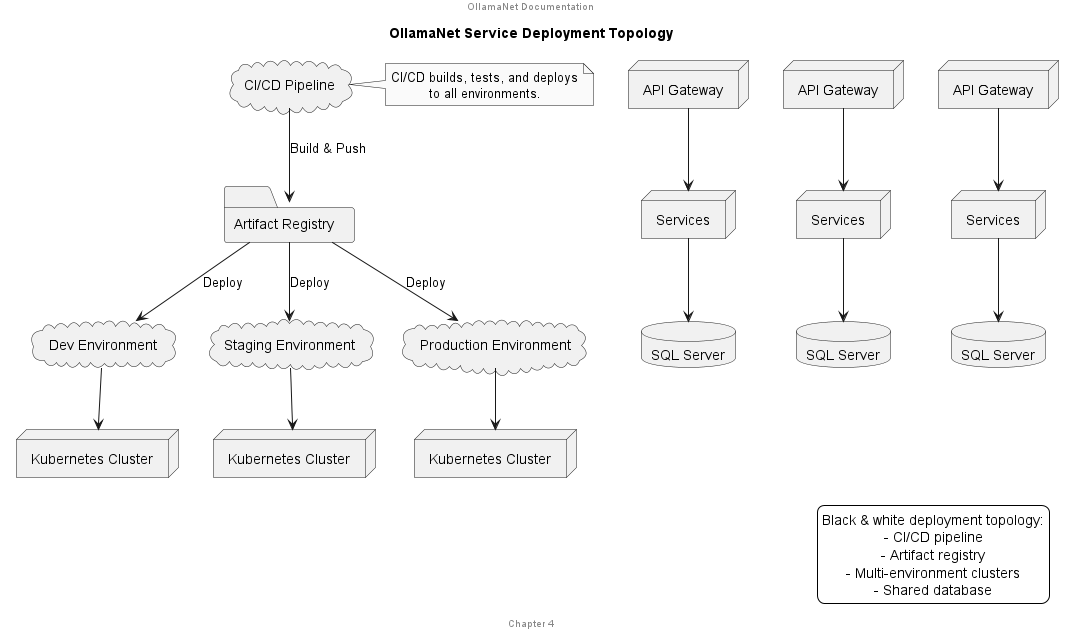
\includegraphics[width=\textwidth]{./Chapter04/figures/service_deployment.png}
    \caption{OllamaNet System Topology and Deployment View}
    \label{fig:system-topology}
\end{figure}
\clearpage

The deployment architecture supports:

\begin{enumerate}
   \item \textbf{Containerization}: All services are containerized for consistent deployment.
   \item \textbf{Horizontal Scaling}: Services can be scaled out by adding instances.
   \item \textbf{Environment Isolation}: Development, testing, and production environments are isolated.
   \item \textbf{Cloud Deployment}: The system can be deployed to various cloud providers.
   \item \textbf{On-Premises Deployment}: The system can also be deployed on-premises.
\end{enumerate}

\subsection{Key Architectural Decisions and Rationales}

\begin{table}[h]
  \centering
  \caption{Key Architectural Decisions and Rationales}
  \label{tab:architectural-decisions}
  \begin{tabular}{|p{0.3\textwidth}|p{0.6\textwidth}|}
    \hline
    \textbf{Decision} & \textbf{Rationale} \\
    \hline
    Microservices Architecture & Enables independent development, deployment, and scaling of components \\
    \hline
    API Gateway Pattern & Provides a single entry point for clients, simplifying client integration \\
    \hline
    Domain-Driven Design & Aligns services with business domains for better maintainability \\
    \hline
    JWT Authentication & Enables stateless authentication across services \\
    \hline
    SQL Server Database & Provides robust relational data storage with strong consistency \\
    \hline
    Redis Caching & Improves performance by caching frequently accessed data \\
    \hline
    RabbitMQ Messaging & Enables asynchronous communication and service discovery \\
    \hline
    Notebook-First Inference & Allows flexible deployment of inference capabilities in cloud environments \\
    \hline
  \end{tabular}
\end{table}

\section{Service Decomposition Strategy}

\subsection{Microservice Boundaries and Responsibilities}

The OllamaNet platform is decomposed into services based on business domains and responsibilities:

\begin{enumerate}
   \item \textbf{Auth Service}
   \begin{itemize}
      \item User registration and authentication
      \item JWT token issuance and validation
      \item Role and permission management
      \item User profile management
   \end{itemize}

   \item \textbf{Admin Service}
   \begin{itemize}
      \item User account administration
      \item AI model management and deployment
      \item Tag and category management
      \item System configuration and monitoring
   \end{itemize}

   \item \textbf{Explore Service}
   \begin{itemize}
      \item AI model discovery and browsing
      \item Search and filtering capabilities
      \item Model metadata presentation
      \item Caching for performance optimization
   \end{itemize}

   \item \textbf{Conversation Service}
   \begin{itemize}
      \item Conversation management and organization
      \item Chat interaction with AI models
      \item Document processing for context enhancement
      \item Folder and organization features
   \end{itemize}

   \item \textbf{Inference Service (Spicy Avocado)}
   \begin{itemize}
      \item AI model inference and response generation
      \item Service discovery via RabbitMQ
      \item Notebook-first architecture for cloud deployment
      \item Integration with Ollama engine
   \end{itemize}

   \item \textbf{Gateway Service}
   \begin{itemize}
      \item Request routing to appropriate services
      \item Authentication and authorization enforcement
      \item Cross-cutting concerns like CORS and rate limiting
      \item Request/response transformation
   \end{itemize}
\end{enumerate}

\subsection{Domain-Driven Design Application}

The service decomposition follows Domain-Driven Design principles:

\begin{enumerate}
   \item \textbf{Bounded Contexts}: Each service represents a distinct bounded context with its own domain model.
   \item \textbf{Ubiquitous Language}: Each service uses consistent terminology within its domain.
   \item \textbf{Aggregates}: Domain entities are organized into aggregates with clear boundaries.
   \item \textbf{Domain Events}: Services communicate through domain events when appropriate.
\end{enumerate}

\begin{figure}[p]
    \centering
    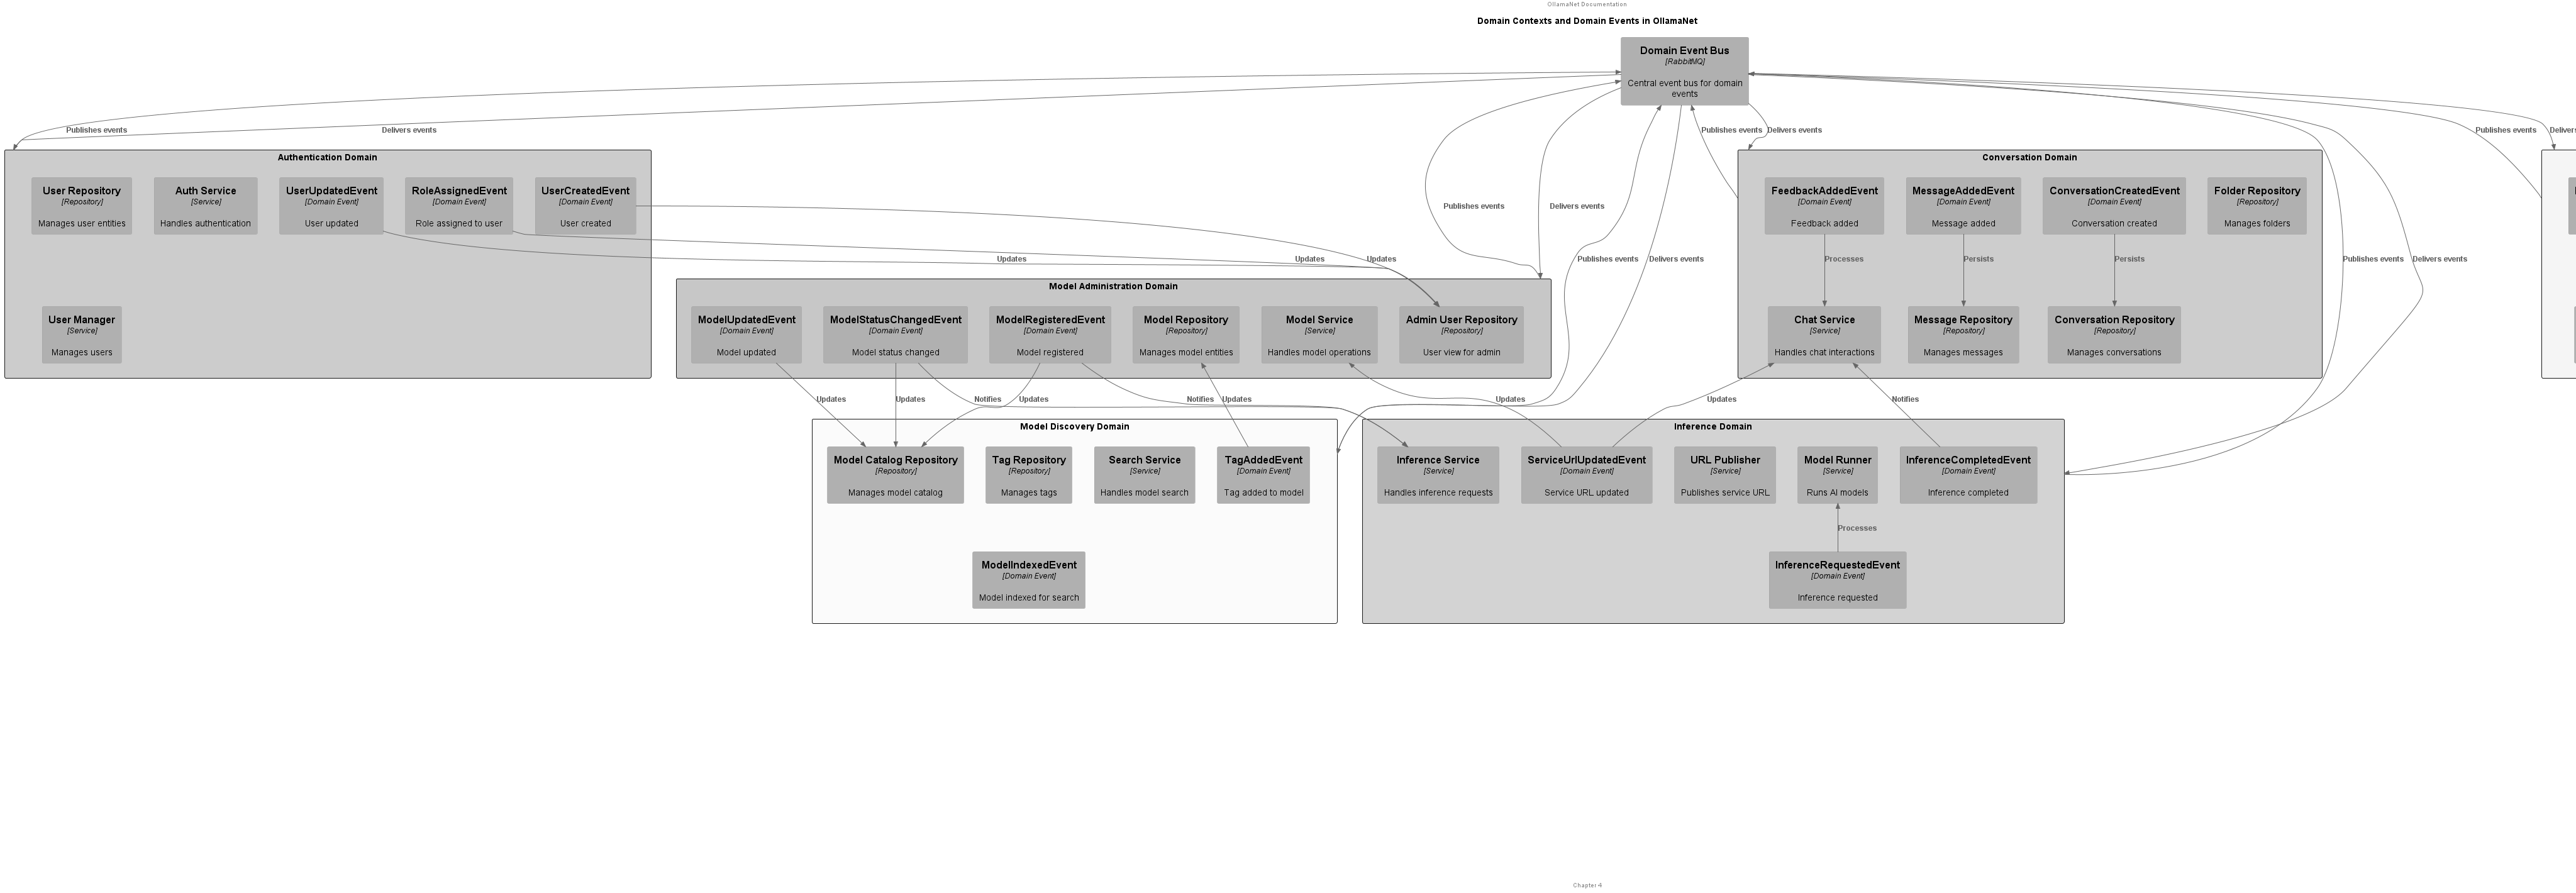
\includegraphics[width=\textwidth]{./Chapter04/figures/domain_contexts.png}
    \caption{OllamaNet Bounded Contexts in Domain-Driven Design}
    \label{fig:domain-contexts}
\end{figure}
\clearpage

\subsection{Service Granularity Decisions}

The service granularity in OllamaNet balances several factors:

\begin{enumerate}
   \item \textbf{Business Domain Alignment}: Services align with distinct business capabilities.
   \item \textbf{Team Ownership}: Services can be owned by specific teams.
   \item \textbf{Deployment Independence}: Services can be deployed independently.
   \item \textbf{Scalability Requirements}: Services can be scaled based on their specific load patterns.
\end{enumerate}

For example, the Inference Service is separated from the Conversation Service because:
\begin{itemize}
   \item It has different scaling requirements (compute-intensive)
   \item It has a unique deployment model (notebook-first architecture)
   \item It integrates with external systems (Ollama engine)
\end{itemize}

\subsection{Service Composition and Dependencies}

Services in OllamaNet have the following dependencies:

\begin{enumerate}
   \item \textbf{Auth Service}: No dependencies on other services
   \item \textbf{Admin Service}: Depends on Auth Service for authentication
   \item \textbf{Explore Service}: Depends on Auth Service for authentication
   \item \textbf{Conversation Service}: 
   \begin{itemize}
      \item Depends on Auth Service for authentication
      \item Depends on Inference Service for AI model responses
   \end{itemize}
   \item \textbf{Inference Service}: No direct dependencies on other services
   \item \textbf{Gateway Service}: Depends on all services for routing
\end{enumerate}

\begin{figure}[p]
    \centering
    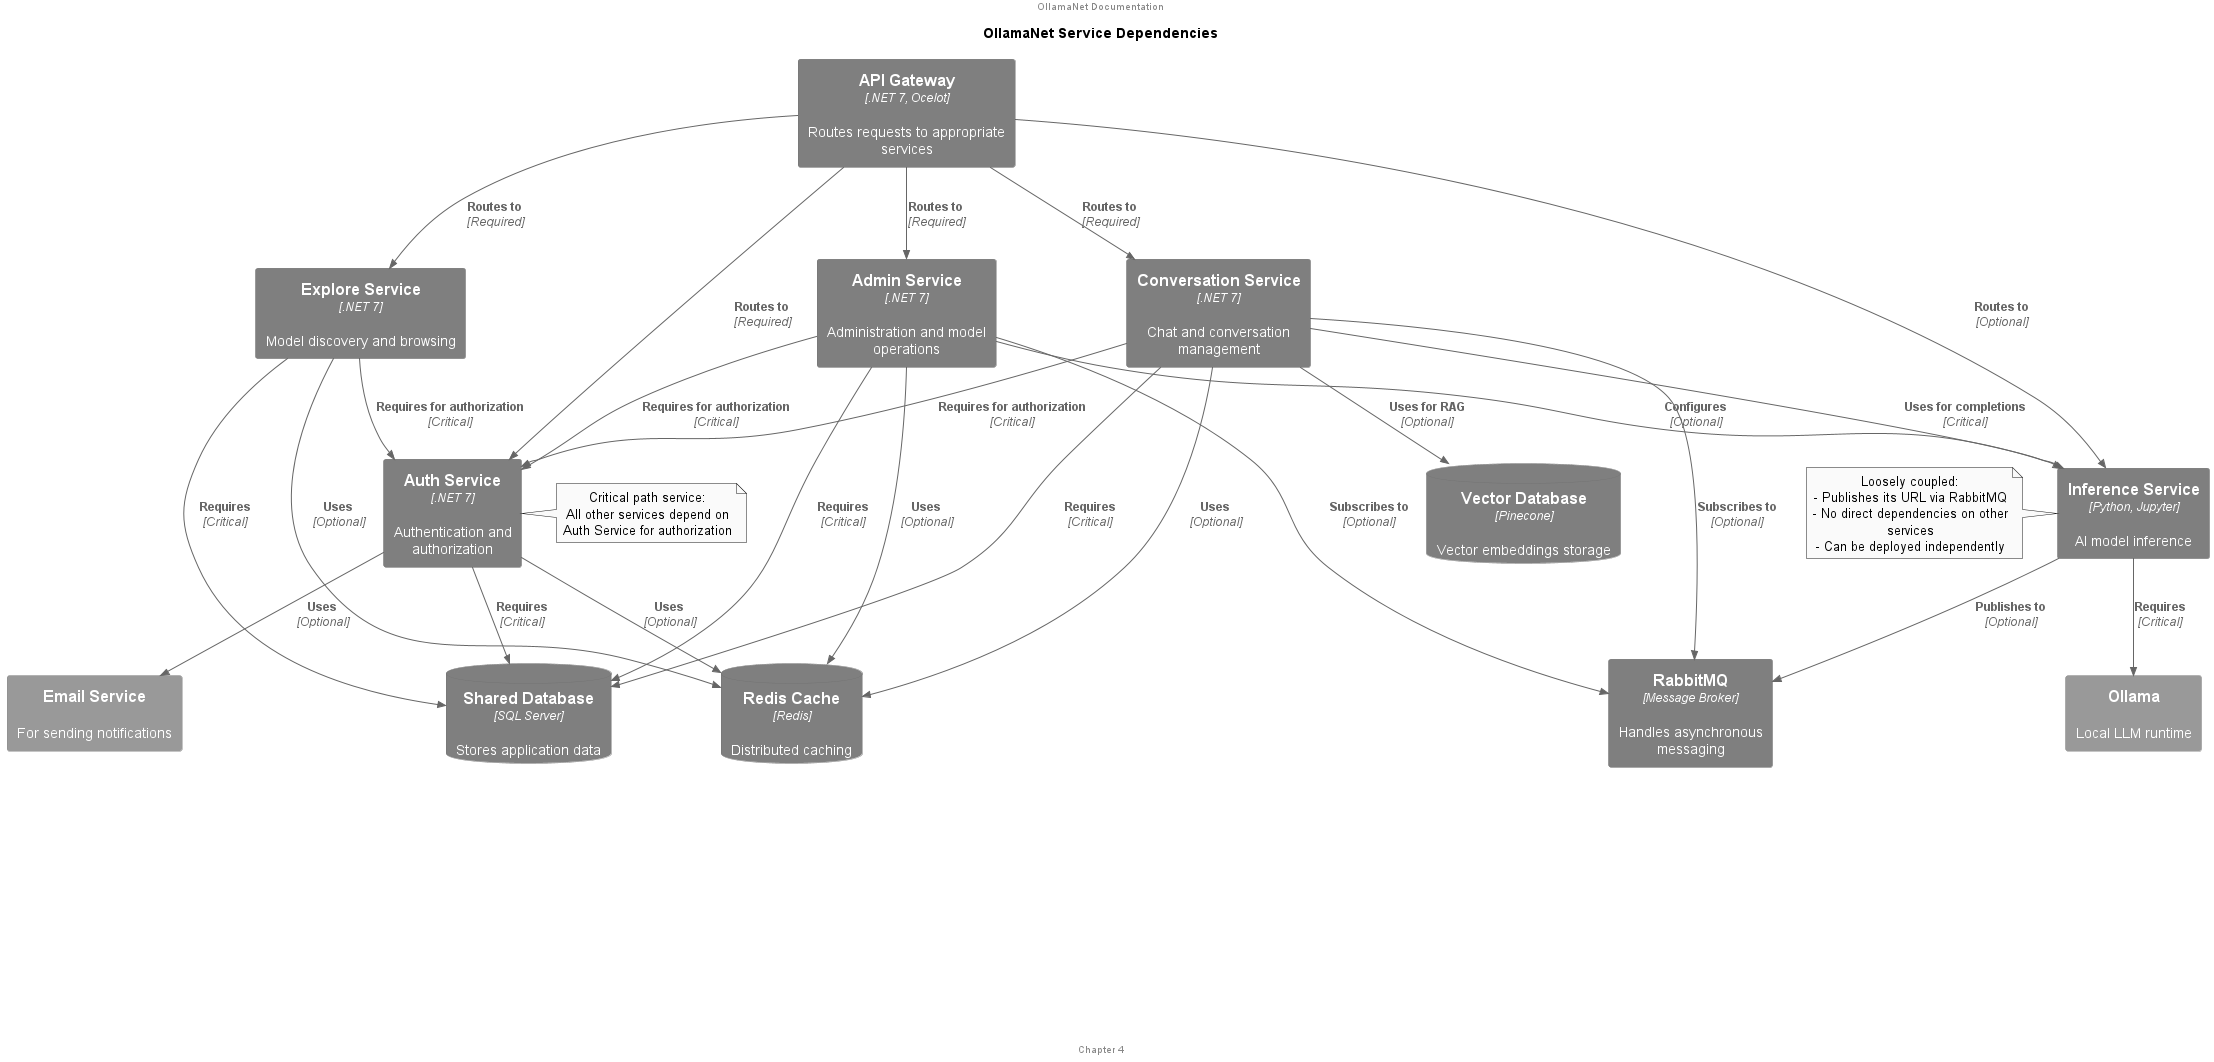
\includegraphics[width=\textwidth]{./Chapter04/figures/service_dependencies.png}
    \caption{OllamaNet Service Dependencies}
    \label{fig:service-dependencies}
\end{figure}
\clearpage

\section{Service Discovery and Registry}

\subsection{Service Discovery Mechanisms}

OllamaNet implements service discovery using RabbitMQ, particularly for the dynamic discovery of Inference Service endpoints:

\begin{enumerate}
   \item \textbf{Publisher-Subscriber Pattern}: Services publish their endpoints to RabbitMQ topics.
   \item \textbf{Topic Exchange}: A "service-discovery" exchange routes messages based on routing keys.
   \item \textbf{Routing Keys}: Structured keys like "inference.url.changed" identify message types.
   \item \textbf{Message Format}: JSON messages contain service URLs and metadata.
\end{enumerate}

\begin{figure}[p]
    \centering
    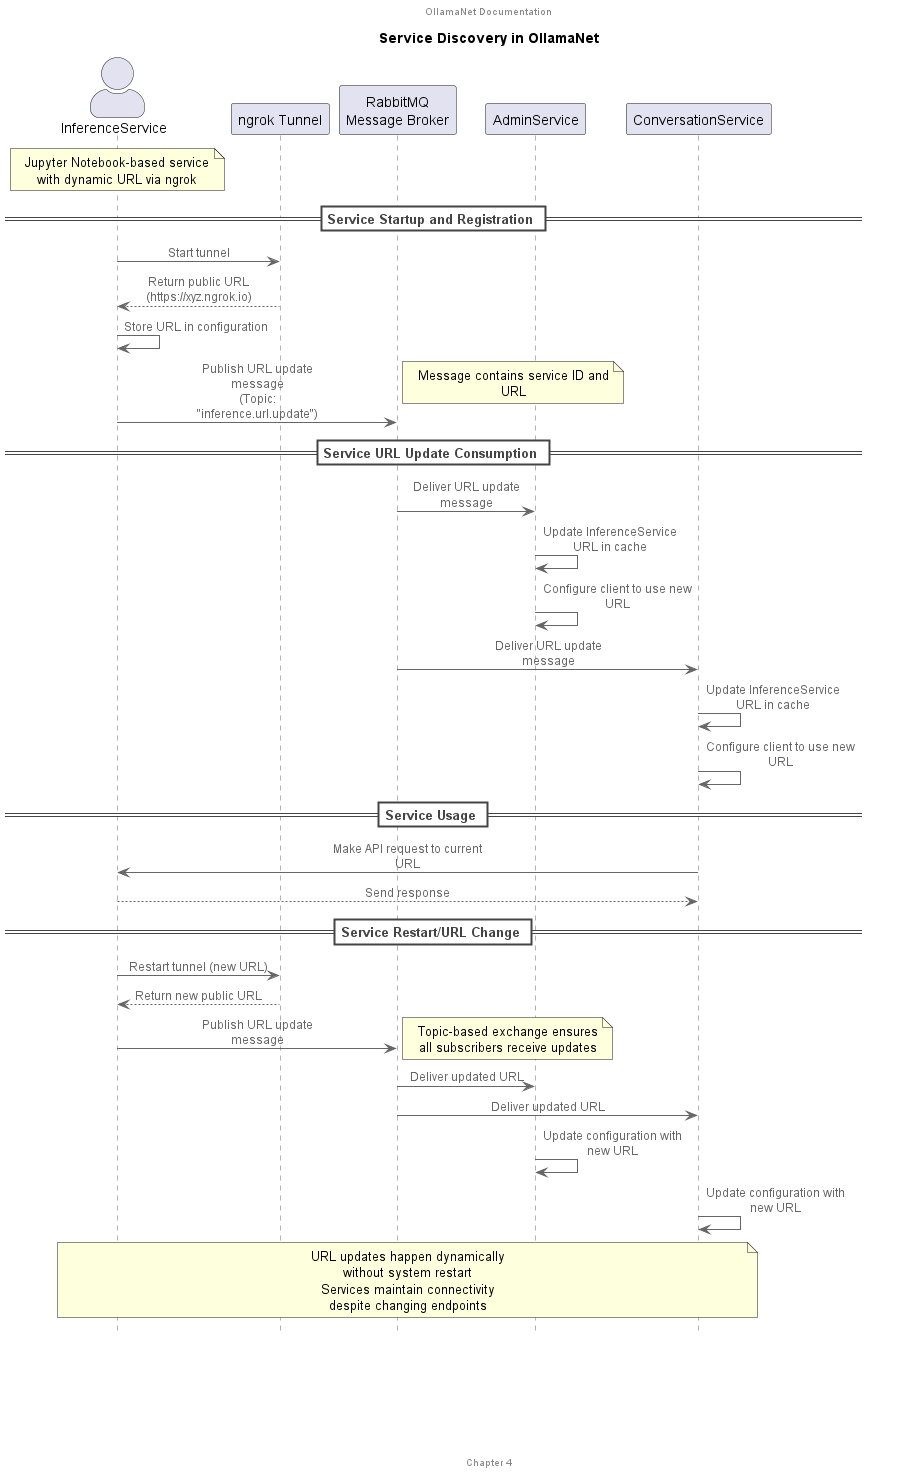
\includegraphics[width=\textwidth]{./Chapter04/figures/service_discovery.png}
    \caption{Service Discovery Sequence Diagram}
    \label{fig:service-discovery}
\end{figure}
\clearpage

\subsection{Dynamic Service URL Configuration}

The system handles dynamic URL configuration through several mechanisms:

\begin{enumerate}
   \item \textbf{Initial Configuration}: Services start with default URLs from configuration files.
   \item \textbf{Runtime Updates}: Services receive URL updates via RabbitMQ messages.
   \item \textbf{Configuration Service}: A central service manages and distributes configuration.
   \item \textbf{Caching}: Updated URLs are cached in Redis for persistence across restarts.
\end{enumerate}

\begin{verbatim}
public async Task UpdateBaseUrl(string newUrl)
{
    if (string.IsNullOrEmpty(newUrl) || _currentBaseUrl == newUrl)
        return;
        
    if (!_urlValidator.IsValid(newUrl))
    {
        _logger.LogWarning("Received invalid URL update: {Url}", newUrl);
        return;
    }
    
    _currentBaseUrl = newUrl;
    await _redisCacheService.SetStringAsync(CACHE_KEY, newUrl);
    _logger.LogInformation("InferenceEngine URL updated to: {Url}", newUrl);
    
    BaseUrlChanged?.Invoke(newUrl);
}
\end{verbatim}

\subsection{Service Registration Approaches}

Services register themselves through different mechanisms:

\begin{enumerate}
   \item \textbf{Static Registration}: Most services have static endpoints defined in configuration.
   \item \textbf{Dynamic Registration}: The Inference Service dynamically registers its endpoint.
   \item \textbf{Health Checks}: Services provide health check endpoints for availability monitoring.
   \item \textbf{Service Metadata}: Registration includes service metadata like version and capabilities.
\end{enumerate}

\subsection{Service Health Monitoring}

The system monitors service health through several approaches:

\begin{enumerate}
   \item \textbf{Health Check Endpoints}: Each service exposes a \texttt{/health} endpoint.
   \item \textbf{Circuit Breakers}: Services implement circuit breakers to detect and handle failures.
   \item \textbf{Heartbeats}: Services send periodic heartbeats to indicate liveness.
   \item \textbf{Logging and Monitoring}: Centralized logging captures service health events.
\end{enumerate}

\section{API Gateway}

\subsection{Gateway Architecture Using Ocelot}

The OllamaNet Gateway is built using the Ocelot API Gateway library, providing a robust and flexible routing solution:

\begin{figure}[p]
    \centering
    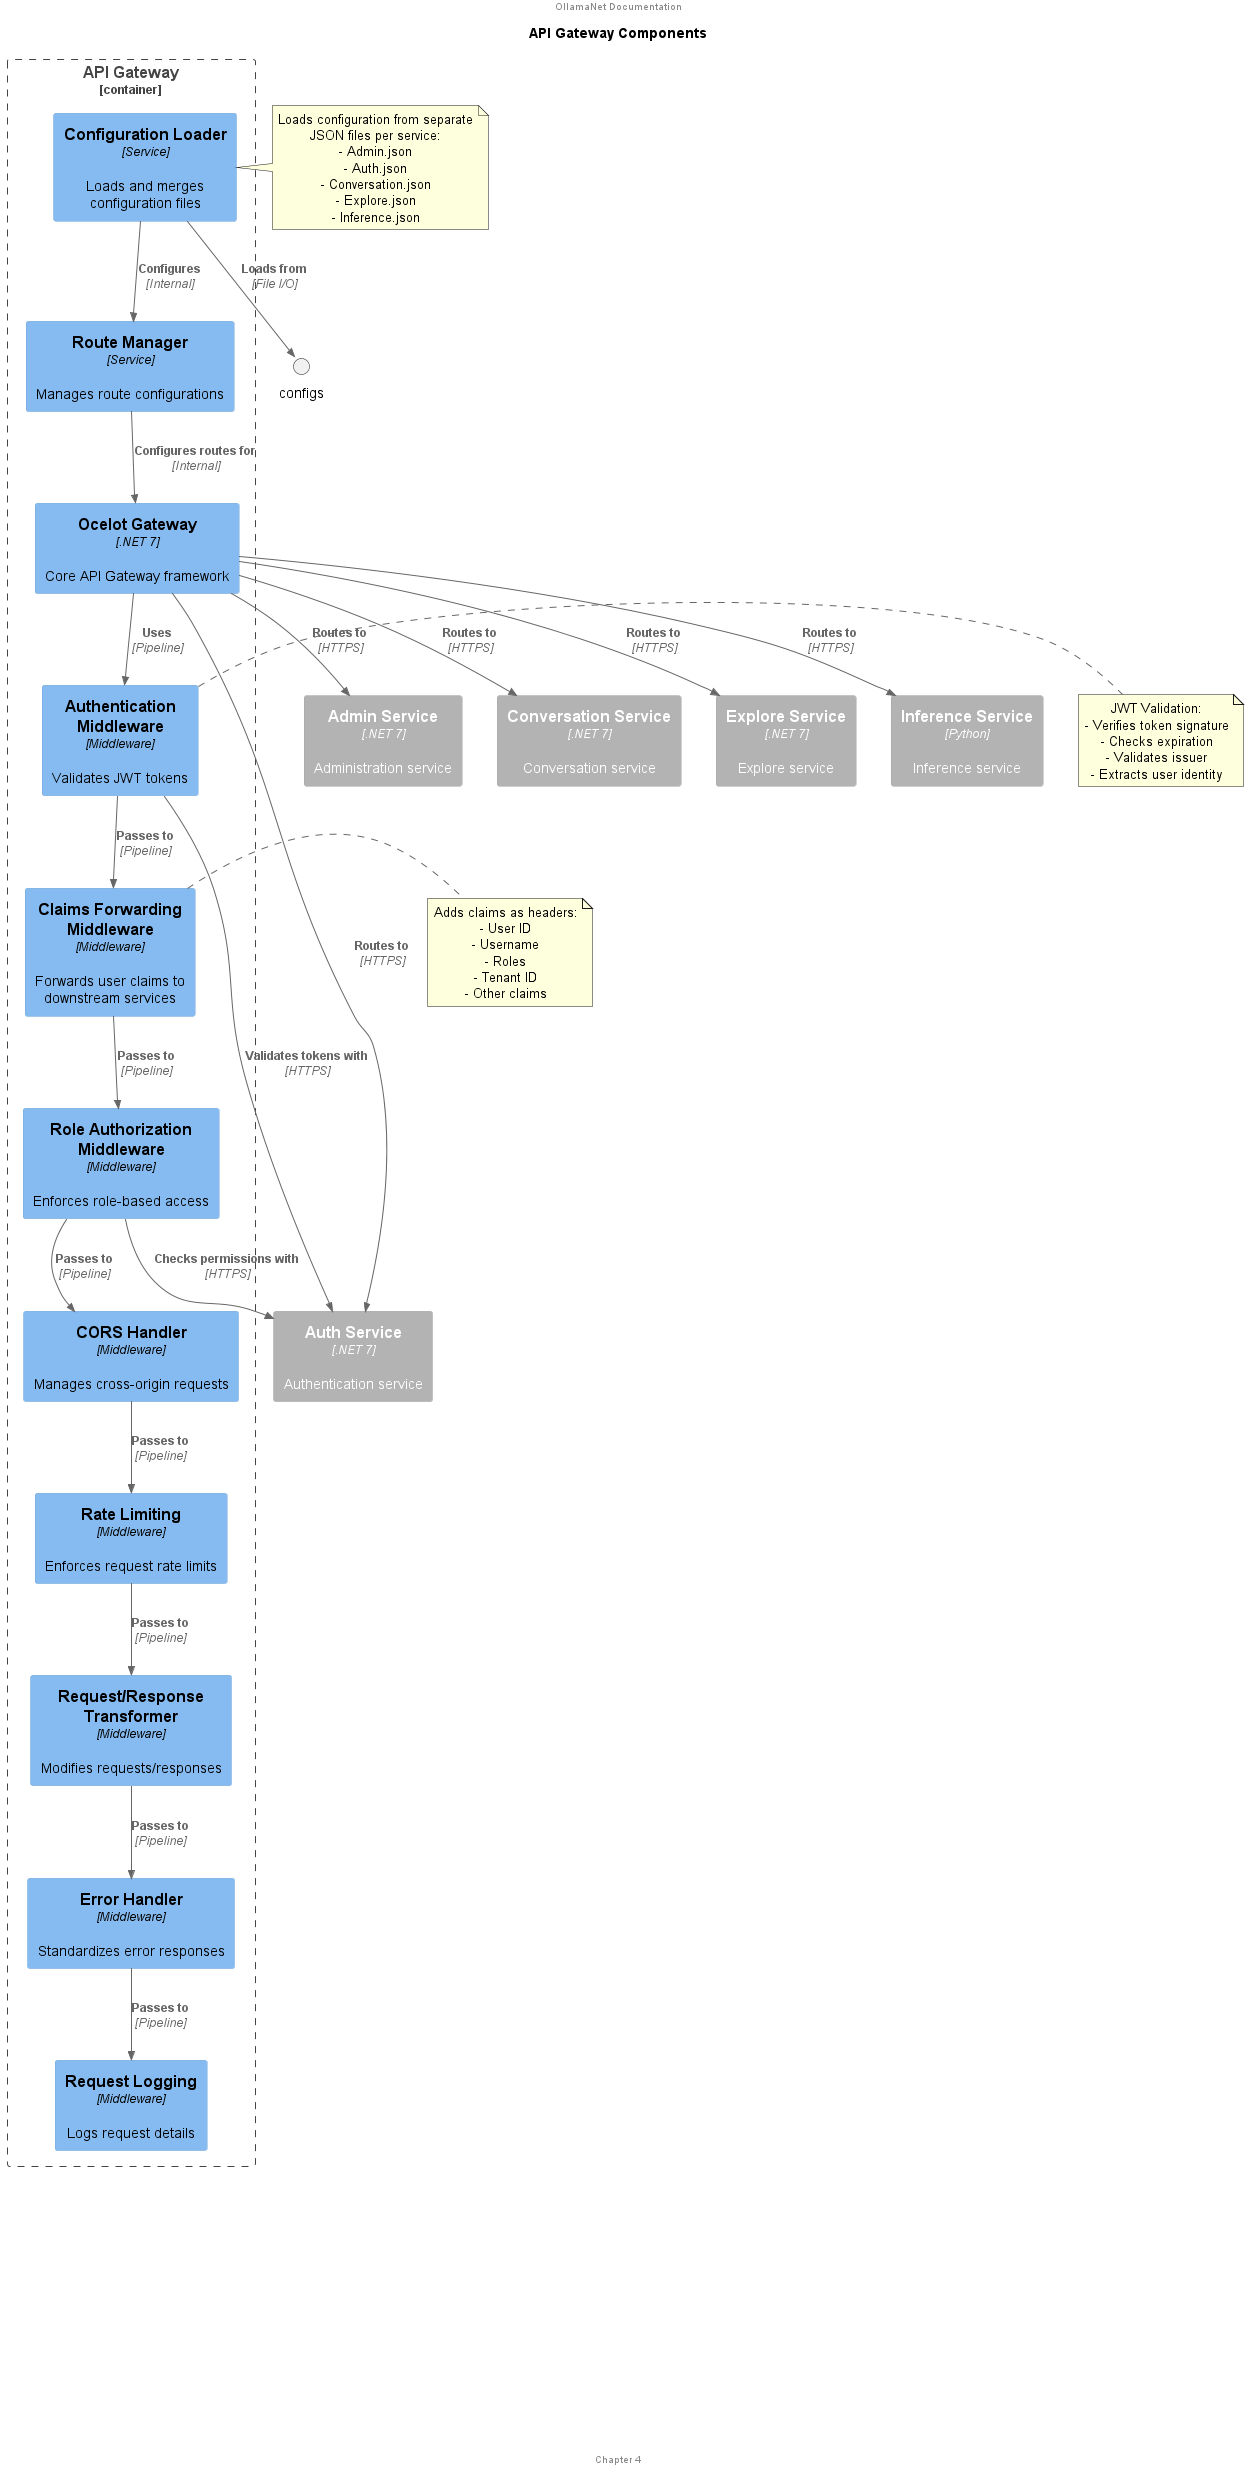
\includegraphics[width=\textwidth]{./Chapter04/figures/gateway_components.png}
    \caption{Gateway Architecture Components}
    \label{fig:gateway-components}
\end{figure}
\clearpage

Key components of the Gateway architecture include:

\begin{enumerate}
   \item \textbf{Ocelot Core}: Handles request routing based on configuration.
   \item \textbf{Middleware Pipeline}: Processes requests through a series of middleware components.
   \item \textbf{Configuration System}: Manages routing and other gateway settings.
   \item \textbf{Authentication Integration}: Validates JWT tokens and enforces security.
\end{enumerate}

\subsection{Routing Configuration and Management}

The Gateway uses a modular configuration approach:

\begin{enumerate}
   \item \textbf{Service-Specific Configurations}: Each service has its own configuration file.
   \item \textbf{Variable Substitution}: Service URLs are defined centrally and referenced via variables.
   \item \textbf{Dynamic Reloading}: Configuration changes are detected and applied without restart.
   \item \textbf{Aggregation}: Individual configurations are combined at runtime.
\end{enumerate}

\begin{verbatim}
{
  "Routes": [
    {
      "DownstreamPathTemplate": "/api/auth/{everything}",
      "DownstreamScheme": "https",
      "DownstreamHostAndPorts": [
        {
          "Host": "${Services.Auth.Host}",
          "Port": 443
        }
      ],
      "UpstreamPathTemplate": "/api/auth/{everything}",
      "UpstreamHttpMethod": [ "GET", "POST", "PUT", "DELETE" ]
    }
  ]
}
\end{verbatim}

\subsection{Authentication and Authorization at Gateway Level}

The Gateway handles authentication and authorization through:

\begin{enumerate}
   \item \textbf{JWT Validation}: Validates tokens issued by the Auth Service.
   \item \textbf{Role-Based Authorization}: Enforces access control based on user roles.
   \item \textbf{Claims Forwarding}: Extracts user claims and forwards them to downstream services.
   \item \textbf{Centralized Policy Enforcement}: Applies consistent security policies across all services.
\end{enumerate}

\begin{verbatim}
public async Task InvokeAsync(HttpContext context)
{
    if (context.User.Identity?.IsAuthenticated ?? false)
    {
        // Extract claims from the authenticated user
        var userId = context.User.FindFirst(ClaimTypes.NameIdentifier)?.Value;
        var email = context.User.FindFirst(ClaimTypes.Email)?.Value;
        var roles = context.User.FindAll(ClaimTypes.Role).Select(c => c.Value);
        
        // Add claims as headers to the request
        if (!string.IsNullOrEmpty(userId))
            context.Request.Headers.Add("X-User-Id", userId);
            
        if (!string.IsNullOrEmpty(email))
            context.Request.Headers.Add("X-User-Email", email);
            
        if (roles.Any())
            context.Request.Headers.Add("X-User-Roles", string.Join(",", roles));
    }
    
    // Continue processing the request
    await _next(context);
}
\end{verbatim}

\subsection{Request/Response Transformation}

The Gateway performs several transformations on requests and responses:

\begin{enumerate}
   \item \textbf{URL Rewriting}: Rewrites URLs based on routing configuration.
   \item \textbf{Header Manipulation}: Adds, removes, or modifies HTTP headers.
   \item \textbf{Response Aggregation}: Combines responses from multiple services when needed.
   \item \textbf{Content Transformation}: Transforms request and response content when required.
\end{enumerate}

\subsection{Cross-cutting Concerns Handled at Gateway}

The Gateway handles several cross-cutting concerns:

\begin{enumerate}
   \item \textbf{CORS}: Configures and enforces Cross-Origin Resource Sharing policies.
   \item \textbf{Rate Limiting}: Prevents abuse by limiting request rates.
   \item \textbf{Logging}: Logs requests and responses for auditing and troubleshooting.
   \item \textbf{Error Handling}: Provides consistent error responses across services.
   \item \textbf{Request Tracing}: Adds correlation IDs for request tracking across services.
\end{enumerate}

\section{Communication Patterns}

\subsection{Synchronous Communication}

\subsubsection{REST API Design and Implementation}

OllamaNet services communicate primarily through RESTful APIs:

\begin{enumerate}
   \item \textbf{Resource-Oriented Design}: APIs are organized around resources.
   \item \textbf{Standard HTTP Methods}: GET, POST, PUT, DELETE are used appropriately.
   \item \textbf{Status Codes}: Proper HTTP status codes indicate success or failure.
   \item \textbf{Content Negotiation}: APIs support multiple content types (primarily JSON).
\end{enumerate}

\begin{verbatim}
[ApiController]
[Route("api/[controller]")]
public class ConversationsController : ControllerBase
{
    [HttpGet]
    public async Task<ActionResult<IEnumerable<ConversationDto>>> GetConversations()
    {
        // Implementation
    }
    
    [HttpGet("{id}")]
    public async Task<ActionResult<ConversationDto>> GetConversation(Guid id)
    {
        // Implementation
    }
    
    [HttpPost]
    public async Task<ActionResult<ConversationDto>> CreateConversation(CreateConversationDto dto)
    {
        // Implementation
    }
    
    // Other endpoints
}
\end{verbatim}

\subsubsection{Request-Response Patterns}

Services implement several request-response patterns:

\begin{enumerate}
   \item \textbf{Synchronous Request-Response}: Client sends a request and waits for a response.
   \item \textbf{Streaming Responses}: Used for real-time AI model responses.
   \item \textbf{Pagination}: Large result sets are paginated for efficiency.
   \item \textbf{Filtering and Sorting}: Clients can specify filters and sort orders.
\end{enumerate}

\subsubsection{HTTP/HTTPS Communication}

All service-to-service communication uses HTTPS with:

\begin{enumerate}
   \item \textbf{TLS Encryption}: All traffic is encrypted using TLS.
   \item \textbf{Certificate Validation}: Services validate certificates for security.
   \item \textbf{Connection Pooling}: HTTP clients use connection pooling for efficiency.
   \item \textbf{Timeout Management}: Appropriate timeouts prevent resource exhaustion.
\end{enumerate}

\subsection{Asynchronous Communication}

\subsubsection{Message Broker Usage (RabbitMQ)}

OllamaNet uses RabbitMQ for asynchronous communication:

\begin{enumerate}
   \item \textbf{Topic Exchange}: Messages are routed based on routing keys.
   \item \textbf{Durable Messaging}: Messages persist across broker restarts.
   \item \textbf{Dead Letter Queues}: Failed messages are sent to dead letter queues for handling.
   \item \textbf{Consumer Acknowledgments}: Messages are acknowledged when processed successfully.
\end{enumerate}

\begin{figure}[p]
    \centering
    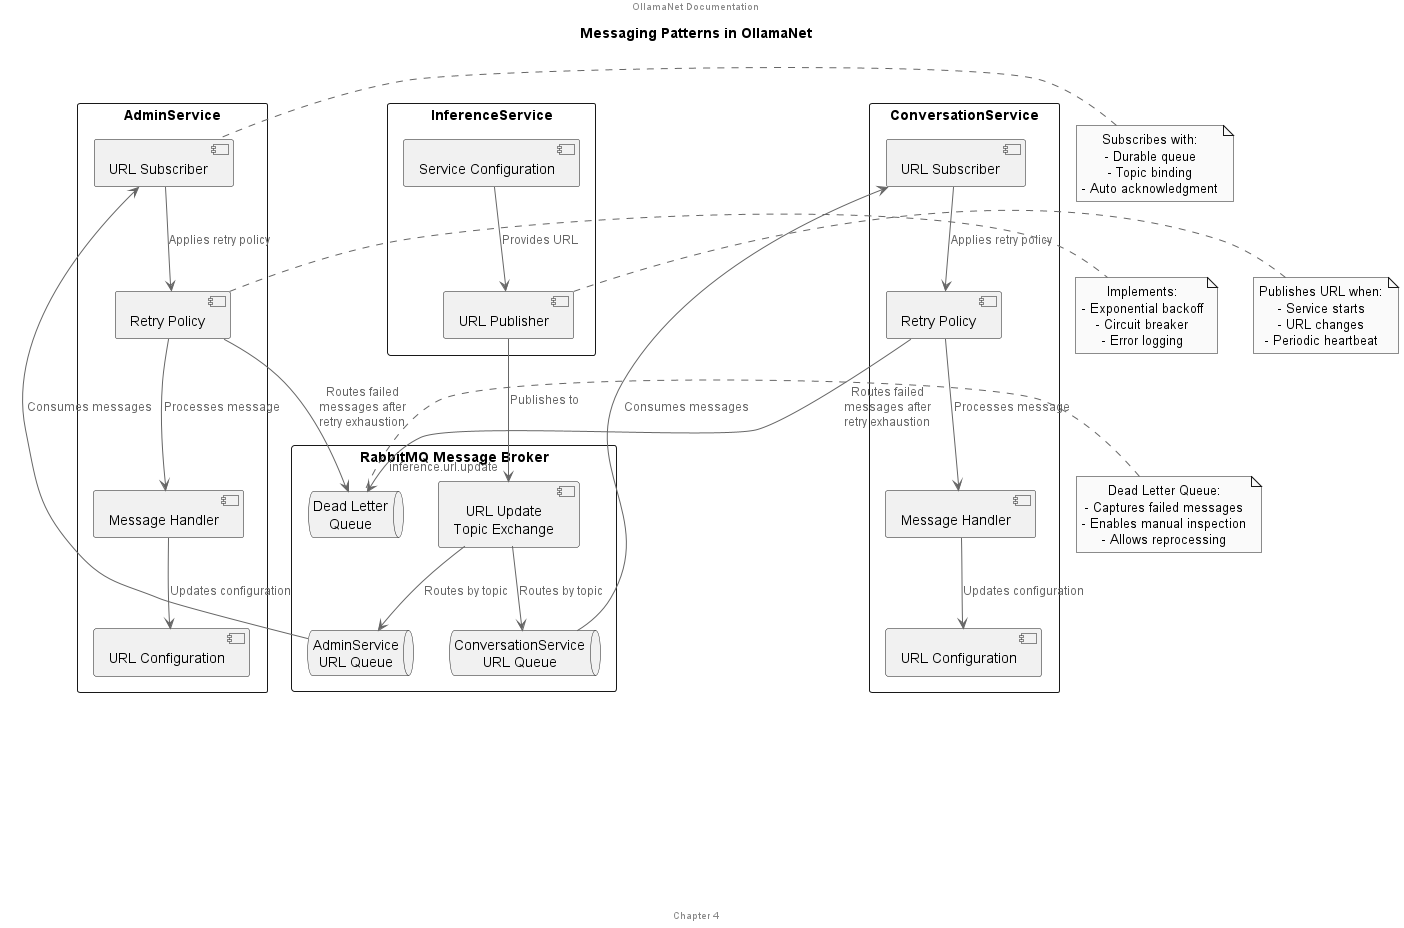
\includegraphics[width=\textwidth]{./Chapter04/figures/messaging_patterns.png}
    \caption{Message Broker Communication Patterns}
    \label{fig:messaging-patterns}
\end{figure}
\clearpage

\subsubsection{Event-Driven Communication}

The system uses event-driven communication for:

\begin{enumerate}
   \item \textbf{Service Discovery}: Inference Service publishes URL updates.
   \item \textbf{State Changes}: Services publish events when important state changes occur.
   \item \textbf{Asynchronous Processing}: Long-running operations use events for completion notification.
   \item \textbf{Integration Events}: Cross-service business processes use events for coordination.
\end{enumerate}

\subsubsection{Message Formats and Standards}

Messages follow these standards:

\begin{enumerate}
   \item \textbf{JSON Format}: All messages use JSON for compatibility.
   \item \textbf{Metadata Inclusion}: Messages include metadata like timestamp and version.
   \item \textbf{Schema Validation}: Messages are validated against schemas.
   \item \textbf{Versioning}: Message formats include version information for compatibility.
\end{enumerate}

\begin{verbatim}
{
  "newUrl": "https://example-inference-engine.ngrok-free.app/",
  "timestamp": "2023-08-15T14:30:00Z",
  "serviceId": "inference-engine",
  "version": "1.0"
}
\end{verbatim}

\subsubsection{Publishing and Subscribing Mechanisms}

The system implements these messaging patterns:

\begin{enumerate}
   \item \textbf{Publish-Subscribe}: One publisher, multiple subscribers.
   \item \textbf{Work Queues}: Tasks distributed among multiple workers.
   \item \textbf{RPC}: Request-reply pattern over messaging.
   \item \textbf{Broadcast}: Messages sent to all interested parties.
\end{enumerate}

\begin{verbatim}
public async Task PublishInferenceUrlUpdate(string newUrl)
{
    var message = new InferenceUrlUpdateMessage
    {
        NewUrl = newUrl,
        Timestamp = DateTime.UtcNow
    };
    
    var factory = new ConnectionFactory
    {
        HostName = _options.HostName,
        Port = _options.Port,
        UserName = _options.UserName,
        Password = _options.Password,
        VirtualHost = _options.VirtualHost
    };
    
    using var connection = factory.CreateConnection();
    using var channel = connection.CreateModel();
    
    channel.ExchangeDeclare(
        exchange: _options.Exchange,
        type: ExchangeType.Topic,
        durable: true);
        
    var json = JsonSerializer.Serialize(message);
    var body = Encoding.UTF8.GetBytes(json);
    
    channel.BasicPublish(
        exchange: _options.Exchange,
        routingKey: _options.InferenceUrlRoutingKey,
        basicProperties: null,
        body: body);
}
\end{verbatim}

\section{Cross-Cutting Concerns}

\subsection{Authentication \& Authorization}

\subsubsection{JWT Implementation}

OllamaNet implements JWT-based authentication:

\begin{enumerate}
   \item \textbf{Token Issuance}: The Auth Service issues JWT tokens upon successful login.
   \item \textbf{Token Validation}: The Gateway and services validate tokens before processing requests.
   \item \textbf{Claims-Based Identity}: Tokens contain claims about the user's identity and roles.
   \item \textbf{Refresh Tokens}: Long-lived refresh tokens enable session persistence.
\end{enumerate}

\subsubsection{Role-Based Access Control}

The system implements role-based access control:

\begin{enumerate}
   \item \textbf{Role Definitions}: Users are assigned roles (Admin, User, etc.).
   \item \textbf{Permission Mapping}: Roles map to permissions for specific operations.
   \item \textbf{Gateway Enforcement}: The Gateway enforces role requirements for routes.
   \item \textbf{Service-Level Checks}: Services perform additional authorization checks as needed.
\end{enumerate}

\begin{verbatim}
{
  "RoleAuthorization": [
    {
      "PathTemplate": "/api/admin/*",
      "RequiredRole": "Admin"
    },
    {
      "PathTemplate": "/api/conversations/*",
      "RequiredRole": "User"
    }
  ]
}
\end{verbatim}

\subsubsection{Claims Forwarding Between Services}

User claims are forwarded between services:

\begin{enumerate}
   \item \textbf{Gateway Extraction}: The Gateway extracts claims from JWT tokens.
   \item \textbf{Header Injection}: Claims are added as HTTP headers to downstream requests.
   \item \textbf{Service Validation}: Services validate and use the forwarded claims.
   \item \textbf{Consistent Identity}: User identity is maintained across service boundaries.
\end{enumerate}

\subsection{Logging \& Monitoring}

\subsubsection{Centralized Logging Approach}

OllamaNet implements centralized logging:

\begin{enumerate}
   \item \textbf{Structured Logging}: All logs use a structured format (JSON).
   \item \textbf{Log Levels}: Appropriate log levels (Debug, Info, Warning, Error) are used.
   \item \textbf{Correlation IDs}: Requests are tracked across services using correlation IDs.
   \item \textbf{Contextual Information}: Logs include relevant context for troubleshooting.
\end{enumerate}

\subsubsection{Monitoring Strategies}

The system is monitored through:

\begin{enumerate}
   \item \textbf{Health Checks}: Services expose health check endpoints.
   \item \textbf{Metrics Collection}: Key performance metrics are collected.
   \item \textbf{Alerting}: Alerts are triggered for critical issues.
   \item \textbf{Dashboard Visualization}: Metrics are visualized in dashboards.
\end{enumerate}

\subsubsection{Observability Features}

Observability is achieved through:

\begin{enumerate}
   \item \textbf{Distributed Tracing}: Requests are traced across service boundaries.
   \item \textbf{Performance Metrics}: Response times, throughput, and error rates are tracked.
   \item \textbf{Resource Utilization}: CPU, memory, and network usage are monitored.
   \item \textbf{Business Metrics}: Key business metrics are tracked for insights.
\end{enumerate}

\subsection{Resilience Patterns}

\subsubsection{Circuit Breaker Patterns}

Circuit breakers prevent cascading failures:

\begin{enumerate}
   \item \textbf{Failure Detection}: Tracks failures in downstream service calls.
   \item \textbf{Open Circuit}: Stops calls to failing services after threshold is reached.
   \item \textbf{Half-Open State}: Allows test calls to check if service has recovered.
   \item \textbf{Closed Circuit}: Normal operation when service is healthy.
\end{enumerate}

\begin{verbatim}
// Configure HTTP client with circuit breaker
services.AddHttpClient<IInferenceEngineConnector, InferenceEngineConnector>()
    .AddPolicyHandler(GetCircuitBreakerPolicy());
    
private IAsyncPolicy<HttpResponseMessage> GetCircuitBreakerPolicy()
{
    return HttpPolicyExtensions
        .HandleTransientHttpError()
        .CircuitBreakerAsync(
            handledEventsAllowedBeforeBreaking: 5,
            durationOfBreak: TimeSpan.FromSeconds(30)
        );
}
\end{verbatim}

\subsubsection{Retry Policies}

Retry policies handle transient failures:

\begin{enumerate}
   \item \textbf{Retry Count}: Specifies how many retries to attempt.
   \item \textbf{Backoff Strategy}: Implements exponential backoff between retries.
   \item \textbf{Retry Triggers}: Defines which errors trigger retries.
   \item \textbf{Timeout}: Sets maximum time for operation with retries.
\end{enumerate}

\begin{verbatim}
private IAsyncPolicy<HttpResponseMessage> GetRetryPolicy()
{
    return HttpPolicyExtensions
        .HandleTransientHttpError()
        .OrResult(msg => msg.StatusCode == System.Net.HttpStatusCode.TooManyRequests)
        .WaitAndRetryAsync(
            retryCount: 3,
            sleepDurationProvider: retryAttempt => TimeSpan.FromSeconds(Math.Pow(2, retryAttempt))
        );
}
\end{verbatim}

\subsubsection{Timeout Management}

The system manages timeouts at multiple levels:

\begin{enumerate}
   \item \textbf{Request Timeouts}: HTTP requests have appropriate timeouts.
   \item \textbf{Operation Timeouts}: Complex operations have overall timeouts.
   \item \textbf{Graceful Degradation}: Services degrade gracefully when timeouts occur.
   \item \textbf{User Feedback}: Users are informed about timeouts when appropriate.
\end{enumerate}

\subsubsection{Fallback Strategies}

Fallback strategies provide alternatives when operations fail:

\begin{enumerate}
   \item \textbf{Cached Data}: Return cached data when live data is unavailable.
   \item \textbf{Default Values}: Use sensible defaults when actual values cannot be retrieved.
   \item \textbf{Degraded Functionality}: Provide limited functionality rather than complete failure.
   \item \textbf{User Notification}: Inform users when fallbacks are used.
\end{enumerate}

\begin{terminology}
\begin{description}
    \item[API Gateway] Component that acts as an entry point for client requests to microservices
    \item[Circuit Breaker] Pattern that prevents cascading failures across services
    \item[JWT] JSON Web Token used for authentication between services
    \item[Microservice] Independent deployable service with a specific domain responsibility
    \item[RabbitMQ] Message broker used for asynchronous communication and service discovery
\end{description}
\end{terminology}